\begin{center}
\large Experimento: \textbf{Polarização de TJBs}
\end{center}


\section{Introdução}

O presente relatório visa detalhar o experimento laboratorial realizado na disciplina laboratório de circuitos eletrônicos no dia 20 de agosto de 2019 sobre polarização de transistores de junção bipolar (TJBs). Esses circuitos permitem criar um nível DC desejado para a polarização do amplificador, pois o sinal a ser amplificado normalmente é oriundo de outro circuito que não se tem a garantia que ele esteja com o nível DC desejado. 

A prática consistia principalmente na medição do ponto de operação dos transistores BC 549B e BC 549C com fatores de multiplicação de corrente de base $\beta$ diferentes, como não havia esses tipos de transistores em laboratório eles foram substituídos pelos transistores BC 547A e BC 547B, assim foi necessário medir seus respectivos $\beta$'s. Após isso, foram montados dois circuitos de polarização, o de polarização fixa e o de polarização de emissor com divisor de tensão, um com e outro sem resistência de degeneração no emissor, e com $V_{CC}$ fixado em +12V, como é mostrado na figura \ref{fig:1}:

\begin{figure}[H] 
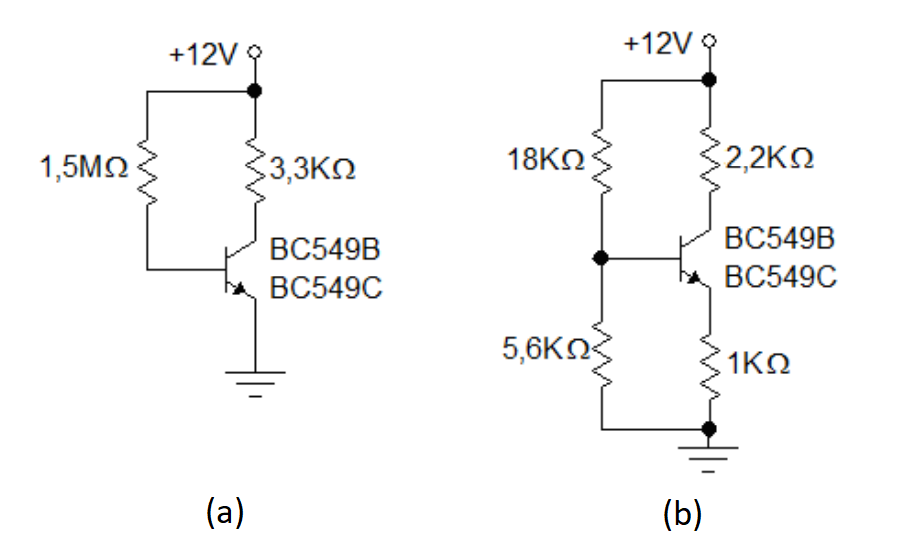
\includegraphics[scale=0.45]{imagens/ckts.png} 
\centering
\caption{Esquema de ligação dos circuitos de polarização: (a) polarização fixa, (b) polarização de emissor com divisor de tensão.}
\label{fig:1} 
\end{figure} 

Com auxílio do multímetro digital da bancada foi medido o ponto de operação $V_{CE}$ e $I_C$ de cada circuito com cada transistor, para se verificar a estabilidade do ponto de polarização do TJB, ou seja analisar se ele encontra no modo de corte, saturado, ou ativo.


\section{Análise teórica}
Inicialmente o $\beta$ dos transistores usados foram medidos por meio de um multímetro, encontrando o valor de 141 para o BC 547A e 281 para o BC 457B.

\subsection{Circuito 1}

A análise inicial será feita para os transistores na configuração do circuito 1, no item (a) da figura \ref{fig:1}. 

Inicialmente supõe-se que o transistor está no modo ativo, assim tem-se que a tensão entre base e emissor pode ser aproximada para:

\begin{center}
    $V_{BE} \approx 0,7 V$
\end{center}

Isso implica que a corrente na base pode ser dada por:

\begin{center}
    $ I_B = \frac{V_{CC}-0,7}{R_B} = 7,533 \mu A$
\end{center}

Assim, a corrente no coletor pode ser encontrada por:

\begin{center}
    $I_C = \beta I_B = \frac{\beta}{R_B} (V_{CC}-0,7)$
\end{center}

Considerando o transistor BC 547A ($I_{C}^{A}$) e o BC 547B ($I_{C}^{B}$), tem-se que a corrente no coletor para cada caso é:

\begin{center}
    $I_{C}^{A} = 1,0621 mA$ e $I_{C}^{B} = 2,1168 mA$
\end{center}

Logo após deve-se encontrar $V_{CE}$ para cada um dos transistores para poder ter a confirmação teórica de que os transistores estão de fato no modo ativo:
 
\begin{center}
    $V_{CE} = V_C - V_E $, com $V_E = 0 => V_{CE} = V_C = V_{CC} - I_C R_C$
\end{center}

Considerando o transistor BC 547A ($V_{CE}^{A}$) e o BC 547B ($V_{CE}^{B}$), tem-se que a tensão entre coletor e emissor para cada caso é:

\begin{center}
    $V_{CE}^{A} = 8,49507 V$ e $V_{CE}^{B} = 5,01456 V$
\end{center}

\subsection{Circuito 2}

A segunda análise será feita para os transistores na configuração do circuito 2, no item (b) da figura \ref{fig:1}.

Adotando a mesma suposição para o valor de $V_{BE}$ e considerando a corrente de base $I_B$ desprezível em relação à corrente que passa pelos resistores de $18k\ohm$ ($R_2$) e $5,6k\ohm$ ($R_1$), obtém-se a tensão de base como:

\begin{center}
    $V_{B} = \frac{R_1}{R_1 + R_2}V_{CC}$
\end{center}

Logo a tensão no emissor é:

\begin{center}
    $V_{E} = V_{B} - V_{BE} = \frac{R_1}{R_1 + R_2}V_{CC} - 0,7$
\end{center}

Desta forma a corrente de emissor é:

\begin{center}
    $I_{E} = \frac{V_E}{R_E} = \frac{\frac{R_1}{R_1 + R_2}V_{CC} - 0,7}{R_E}$
\end{center}

Considerando $\beta$ muito grande, pode aproximar a corrente do coletor como a corrente do emissor, assim:

\begin{center}
    $I_{C} = I_{E}$
\end{center}

Dessa forma, as correntes que passam pelo coletor nos circuitos com os transitores BC 547A ($I_{C}^{A}$) e BC 547B ($I_{C}^{B}$), são:

\begin{center}
    $I_{C}^{A} = I_{C}^{B} = 2,1474 mA$ 
\end{center}

Agora basta encontrar os valores de $V_{CE}$ para cada um dos transistores por meio da expressão:

\begin{center}
    $V_{CE} = V_{CC} - (R_C+R_E)I_C$
\end{center}

Assim, com a mesma nomenclatura que o circuito anterior, tem-se:

\begin{center}
    $V_{CE}^{A} = V_{CE}^{B} = 5,1283 V$
\end{center}


\section{Resultados e discussão}

Os resultados obtidos foram coletados através do multímetro digital da bancada e posto na tabela 2 de valores medidos de $V_{CE}$ e $I_C$ para ambos os circuitos. Primeiramente foi coletado os valores do parâmetro $\beta$ dos transistores BC 547A e BC 547B, que são respectivamente 141 e 281. 

Foi feita uma tabela somente com os valores teóricos obtidos através das equações da análise teórica para facilitar a comparação a ser feita. Pode-se se notar que os valores medidos se aproximaram bastante dos valores teóricos apresentados corroborando toda a atividade realizada.

Para que os transistores possam atuar no modo ativo, as seguintes condições devem ser estabelecidas:

\begin{center}
    $V_{CE}^{x} \geq V_{BE}^{x}$ e $I_{C}^{x} > 0$
\end{center}

Como ambas as condições são atendidas para cada um dos transistores em cada um dos circuitos, então a hipótese inicial de que os transistores estavam no modo ativo se prova verdadeira. Isso se aplica tanto para os valores teóricos como os práticos.

\begin{table}[H]
\centering
\begin{tabular}{l|c|c||c|c|}
\cline{2-5}
\multirow{2}{*}{} & \multicolumn{2}{c||}{{\begin{tabular}[c]{@{}c@{}}
\textbf{Circuito 1}\\ Polarização fixa\end{tabular}}} & 
\multicolumn{2}{c|}{{\begin{tabular}[c]{@{}c@{}}
\textbf{Circuito 2}\\ Polarização de emissor com\\ divisor de tensão\end{tabular}}} \\ 
\cline{2-5} 
&\multicolumn{1}{l|}{\textbf{VCE}} &\textbf{IC} & \textbf{VCE} & \textbf{IC}   \\ \hline
\multicolumn{1}{|c|}{\textbf{BC547A}} & 8.49 V  & 1.06 mA  & 5.12 V & 2.14 mA  \\ \hline
\multicolumn{1}{|c|}{\textbf{BC547B}} & 5.01 V  & 2.11 mA   & 5.12 V & 2.14 mA   \\ \hline
\end{tabular}
\caption{Valores teóricos dos circuitos 1 e 2.} 
\end{table}


Além disso é possível fazer um paralelo entre os circuitos de polarização fixa e de polarização de emissor com divisor de tensão, no qual percebe-se que, no esquema de polarização fixa não é tão confiável para os objetivos propostos, tendo que a mudança do valor de $\beta$ muda drasticamente os valores de operação. 

Por outro lado no esquema polarização de emissor com divisor de tensão é possível perceber que $\beta$ tem pouca ou nenhuma influência no ponto de operação, pois os valores do ponto de operação ($I_C$ e $V_{CE}$) não mudam alterando os valores de $\beta$.  

\begin{table}[H]
\centering
\begin{tabular}{l|c|c||c|c|}
\cline{2-5}
\multirow{2}{*}{} & \multicolumn{2}{c||}{{\begin{tabular}[c]{@{}c@{}}
\textbf{Circuito 1}\\ Polarização fixa\end{tabular}}} & 
\multicolumn{2}{c|}{{\begin{tabular}[c]{@{}c@{}}
\textbf{Circuito 2}\\ Polarização de emissor com\\ divisor de tensão\end{tabular}}} \\ 
\cline{2-5} 
&\multicolumn{1}{l|}{\textbf{VCE}} &\textbf{IC} & \textbf{VCE} & \textbf{IC}   \\ \hline
\multicolumn{1}{|c|}{\textbf{BC547A}} & 8.59 V  & 1.05 mA  & 5.15 V & 2.14 mA  \\ \hline
\multicolumn{1}{|c|}{\textbf{BC547B}} & 5.32 V  & 2.04 mA   & 5.11 V & 2.16 mA   \\ \hline
\end{tabular}
\caption{Valores medidos dos circuitos 1 e 2.} 
\end{table}

Verifica-se também que o circuito de polarização de emissor com divisor de tensão é melhor que o circuito de polarização fixa mantendo o ponto de operação com baixa flutuação independente do transistor, pois devido a corrente que passa por $R_E$ vai ter uma queda de tensão que irá ajudar para melhor definir $I_C$, pois a tensão de base $V_B$ vai sofrer maior influência dessa tensão no emissor $V_E$ que não mais estará aterrado diretamente. Porém este circuito obriga a utilizar um resistor de degeneração que ocasiona redução do ganho. Mas este resistor no emissor no circuito 2 vai contribuir para uma estabilidade térmica do circuito.

\section{Conclusões}

Nesta prática foram estudados dois circuitos tradicionais de polarização de TJBs, compreendendo como realizar sua montagem e entendendo os benefícios de utilizar o circuito de polarização de emissor com divisor de tensão em contraste com o de polarização fixa, bem como identificando seus defeitos.

\newpage

\section{Anexos}
Vide em anexo abaixo as folhas de cálculo utilizadas durante o experimento:

\begin{figure}[h!] 
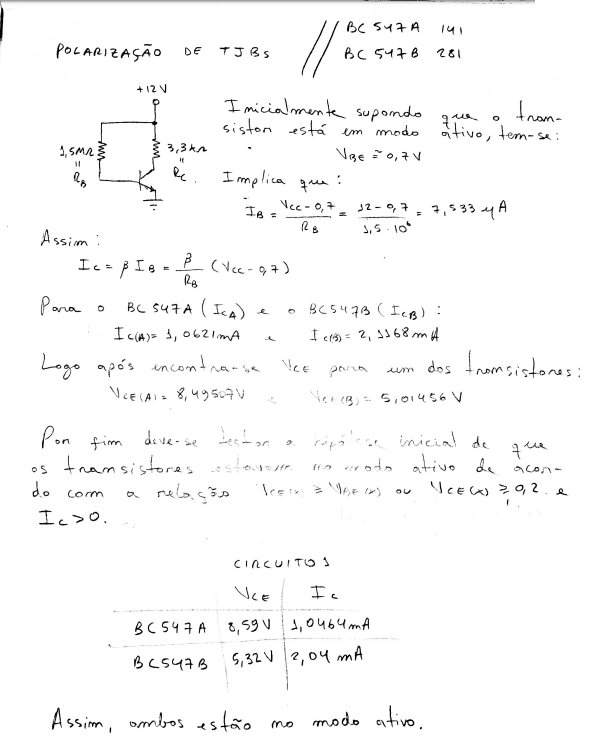
\includegraphics[scale=1]{imagens/calc1.png} 
\centering
\caption{Primeira folha de cálculos.}
\label{calc:1} 
\end{figure} 

\begin{figure}[h!] 
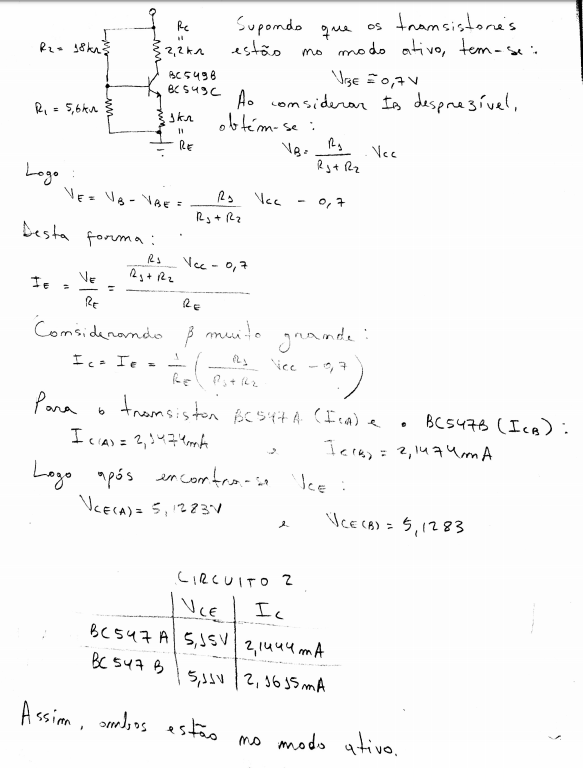
\includegraphics[scale=1]{imagens/calc2.png} 
\centering
\caption{Segunda folha de cálculos.}
\label{calc:2} 
\end{figure} 







     






